
\begin{tikzpicture}[node distance=2cm, auto]
    % Nodes
    \node [draw, rectangle, minimum width=2cm, minimum height=1cm, align=center, label=above:$x(t)$, label=below:Stimulus] (stimulus) {\includegraphics[scale=0.15]{IMAGES/BACKGROUND/stim.pdf}};
    
    \node [draw, fill=blue!20, rectangle,  minimum width=11.5cm, minimum height=5cm, right=0.5cm of stimulus, label=above:\textbf{GLM} ] (GLM_Box) {};

    \node [draw, fill=white, rectangle,  minimum width=2.5cm, minimum height=2.5cm, right=1cm of stimulus, align=center, label=above:$k$, label={[align=center]below:Feedforward \\ filter}] (k) {\includegraphics[scale=0.1]{IMAGES/BACKGROUND/kfilter.pdf}};

   \node [draw, fill=white, circle, right=0.5cm of k, align=center] (plus) {+};

    \node [draw, fill=white, rectangle, minimum width=1cm, minimum height=1cm, above=0.5cm of plus, align=center ,label={[align=center]above:Constant}] (cst) {C};
    
    \node [draw, fill=white, rectangle,  minimum width=2.5cm, minimum height=2.5cm, right=0.5cm of plus, align=center, label=above:$f$, label={[align=center]below:Nonlinear \\ function}] (f) {\includegraphics[scale=0.1]{IMAGES/BACKGROUND/ffunction.pdf}};

    \node [draw, fill=white, rectangle,  minimum width=2.5cm, minimum height=2.5cm, right=1cm of f, align=center, label=above:, label={[align=center]below:Stochastic \\ process}] (Aleatoire) {\includegraphics[scale=0.2]{IMAGES/BACKGROUND/Stocha_process.jpg}};

    \node [draw, rectangle,  minimum width=2cm, minimum height=1cm, right=1cm of Aleatoire, align=center, label=above:$y(t)$, label=below:Responses ] (y) {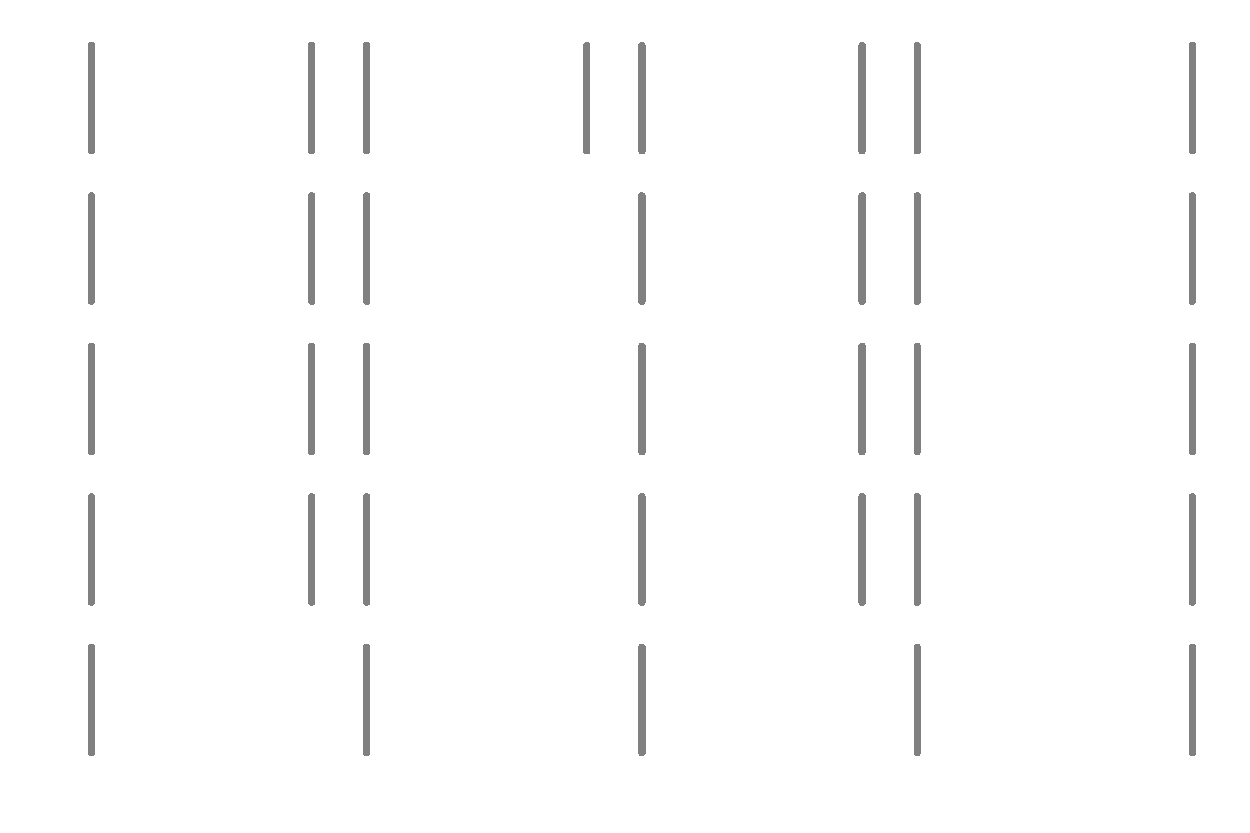
\includegraphics[scale=0.1]{IMAGES/BACKGROUND/y_out.pdf}};
    

    % Arrows
    \draw [->] (stimulus) -- (k);
    \draw [->] (k) -- (plus);
    \draw [->] (plus) -- (f);
    \draw [->] (cst) -- (plus);

  %  \path (A) edge[->] node[above] {Text Above} (B);

    \draw [->] (f) -- node[above] {$\lambda (t)$} (Aleatoire);
    \draw [->] (Aleatoire) -- (y);

  
\end{tikzpicture}


% \node (V1) [V] {V1};
% \node (V2) [V, right of=V1] {V5};
% \node (PPC) [P, above of=V2,xshift = -2cm] {PPC};

% \draw [arrow] (V1) to [bend left=20] (V2);
% \draw [arrow] (V1) to [bend left=20] (PPC);
% \draw [arrow] (V2) to [bend left=20] (V1);
% \draw [arrow] (V2) to [bend left=20] (PPC);
% \draw [arrow] (PPC) to [bend left=20] (V1);
% \draw [arrow] (PPC) to [bend left=20] (V2);

% \node (arrowhead) at (PPC) {}; 
% \node (arrowhead_V1_V2) at (PPC) {}; 
% \draw [-Stealth, dashed] (arrowhead) -- ++(0,-3.5);
% \node (PPC) [P, above of=V2,xshift = -2cm] {PPC};

% \node (Photic) [Photic, below of=V1, yshift = 2cm] {Photic effect};
% \node (Motion) [Motion, below of=V2, yshift = 2cm] {Motion effect};
% \node (Attention) [Attention, right of=PPC] {Attention effect};
